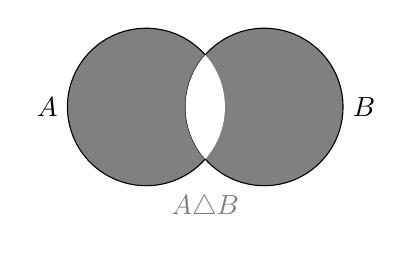
\begin{tikzpicture}
\def\firstcircle{(0,0) circle (1)}
\def\secondcircle{(1.5,0) circle (1)}

\draw[fill=gray] \firstcircle;
\draw[fill=gray] \secondcircle;

\node at (-1,0) [left] {$A$};
\node at (2.5,0) [right] {$B$};

\begin{scope}
\clip \firstcircle;
\fill[white] \secondcircle;
\end{scope}

\node[color=gray] at (0.75,-1) [below] {$A \triangle B$};
\end{tikzpicture}
